Im folgenden soll die Funktionsweise als auch Einbindung ins Projket des XOR-Matchers genauer betrachtet werden.

\subsubsection*{Grundidee des XOR matchers}

Der XOR-Edge-Matcher basiert auf der Überlagerung der Binärmasken zweier Puzzelkanten \ref{fig:xor_idea}. Ziel ist es, durch Rotation und Verschiebung der Kanten eine minimale Überlappung und den geringsten Leerraum zu erreichen. Diese Methode berücksichtigt ausschließlich geometrische Aspekte des Puzzels, ohne Farben oder Muster der Puzzelteile zu berücksichtigen.

\begin{figure}
    \centering
    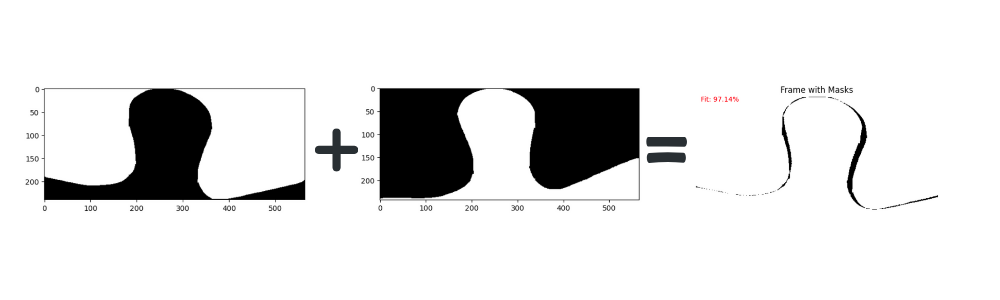
\includegraphics[width=1\linewidth]{sections//solver//images/xor_basic_idea.png}
    \caption{Grundidee des XOR Matchers}
    \label{fig:xor_idea}
\end{figure}

\subsubsection*{Vorbereitung der Daten}

Die Datenvorbereitung umfasst die Umwandlung einer Kantenrepräsentation in eine Binärmaske. Dafür sind mehrere Zwischenschritte notwendig:

\paragraph{1. Normalisierung}
Die Ausrichtung der Kanten variiert. Sie können horizontal oder vertikal mit unterschiedlichen Abständen zum Rand angeordnet sein. Um verwendbare Binärmasken zu generieren, müssen diese Abweichungen normalisiert werden. Dies beinhaltet die Rotation der Kanten um 90°, falls nötig, und die anschließende Verschiebung an den oberen linken Bildrand. Die Notwendigkeit einer Rotation wird durch den Vergleich der Varianz entlang der x- und y-Achse bestimmt:

\[
\operatorname{Var}(x) < \operatorname{Var}(y) \implies \text{vertikale Kante}
\]
\[
\operatorname{Var}(x) > \operatorname{Var}(y) \implies \text{horizontale Kante}
\]
Die Rotation wird durch eine Achsenvertauschung gefolgt von einer Spiegelung entlang der x-Achse durchgeführt:
\[
B = S_x A^T
\]
wobei
\[
S_x = \begin{pmatrix} 1 & 0 \\ 0 & -1 \end{pmatrix}
\]
die Spiegelungsmatrix entlang der x-Achse ist und \( A^T \) die transponierte Matrix von \( A \) darstellt.
Die Matrix \(A\) repräsentiert dabei das Eingangsbild, wobei die Kante mit dem Wert 1 dargestellt wird, und der Rest mit dem Wert 0.

\paragraph{2. Binärmasken}
Die normalisierten Kanten werden anschließend gefüllt. Nach verschiedenen Experimenten mit Techniken wie ``fillPoly'' von OpenCV und ``floodFill'' von scikit-image, wurde ein eigener Füllalgorithmus entwickelt. Die Binärmasken werden von oben nach unten gefüllt, wobei die Kante genau ein Pixel breit sein muss. Ein x-zu-y-Mapping identifiziert den letzten zusammenhängenden weißen Pixel jeder Zeile als Kantenpixel. Der Füllvorgang wechselt die Farbe beim Erreichen einer Kante zwischen Weiß (1) und Schwarz (0). Der Algorithmus wird in Abbildung \ref{alg:maskenfuellung} detaillierter erklärt.
\begin{algorithm}
\caption{Maskenfüllungsalgorithmus}
\label{alg:maskenfuellung}
\begin{algorithmic}[1]
\State \textbf{Input:} BildMaske, KantenMapping
\State \textbf{Output:} GefüllteMaske

\State Initialisiere GefüllteMaske mit den Abmessungen von BildMaske
\State Setze alle Pixel von GefüllteMaske auf 0 (Schwarz)

\For{Jede Spalte $y$ von oben nach unten}
    \State $farbe \gets 1$  \Comment{Startfarbe Weiß}
    \For{Jedes Pixel $x$ in Spalte $y$}
        \If{$x$ ist in KantenMapping für $y$}
            \State $farbe \gets 1 - farbe$  \Comment{Wechselt zwischen 0 und 1}
        \EndIf
        \State Setze Pixel $(x, y)$ in GefüllteMaske auf $farbe$
    \EndFor
\EndFor

\State \textbf{return} GefüllteMaske
\end{algorithmic}
\end{algorithm}

Bei der Auswertung der Ergebnisse wurde festgestellt, dass der Algorithmus Schwierigkeiten bei der Verarbeitung der Scheitelpunkte der Konturen aufweist. Um diese Bildfehler zu korrigieren, wird folgender Ansatz verfolgt: Wenn ein Pixel und seine beiden horizontal benachbarten Pixel unterschiedliche Werte aufweisen, wird das betrachtete Pixel an die Farbe seiner Nachbarn angeglichen.

Der aktuelle Verarbeitungsschritt berücksichtigt nicht, ob es sich bei den Kanten um männliche oder weibliche Typen handelt. Es ist jedoch notwendig, die Binärmaske entsprechend dem im Edge-Objekt definierten Kantentyp anzupassen. Dies geschieht durch die Auswertung der Randpixel: Überwiegen weiße Pixel, handelt es sich vermutlich um eine weibliche Kante; ein Überschuss an schwarzen Pixeln deutet auf eine männliche Kante hin. Stimmt der erkannte Kantentyp nicht mit dem gespeicherten Typ überein, wird das Bild invertiert – weiße Pixel werden schwarz und umgekehrt.

Während des Optimierungsschritts werden die Masken korrekt positioniert und gegebenenfalls leicht rotiert. Hierbei kann ein kleiner schwarzer Rand entstehen, der jedoch nicht als Fehler betrachtet werden sollte. Um mögliche visuelle Störungen zu minimieren, wird zusätzlich ein Padding am Rand der Maske hinzugefügt, um die Darstellung zu verbessern.

\subsubsection*{Optimierung}

Nun geht es um die eigentliche XOR-Optimierung. Dieser Schritt besteht im Grunde aus folgenden sich wiederholenden Schritten:

\paragraph{Masken in Frame platzieren}
Als erstes werden die beiden Binärmasken in einem Frame platziert. Dabei wird die Binärmaske der weiblichen Kante am oberen Rand platziert, und die Maske der männlichen Kante wird so platziert, dass sie bereits etwas mit der weiblichen Binärmaske überlappt. Diese Überlappung wird mit XOR berechnet.

\paragraph{Fit berechnen}
Um nun den Fit zu berechnen werden alle weißen und schwarzen Pixel gezählt. Daraus wird der Score mit dieser Formel berechnet:
\[
1 -  \frac{\left|AnzahlSchwarzerPixel\right|}{\left|AnzahlWeißerPixel\right|}
\]

\paragraph{Verschieben und Rotieren}
Zur Verbesserung des Übereinstimmungsscores wird die Position und Orientierung der Masken durch geringfügiges Verschieben und Rotieren feinjustiert. Dieser Prozess wird so lange fortgesetzt, bis keine weitere Verbesserung des Scores möglich ist, was auf das Erreichen eines lokalen Minimums hinweist. In idealen Fällen entspricht dieses lokale Minimum einem globalen Minimum, allerdings ist die Überprüfung dieser Annahme zeitintensiv und nicht unmittelbar realisierbar.

\subsubsection*{Einbindung in Solver}
Der XOR-Optimierer ist, wie auch die anderen Matcher, über das Matcher-Interface in das Projekt integriert. 

\subsubsection*{Bewertung des Matchers}
Die Auswertung des Beispiel-Puzzles zeigte, dass der XOR-Optimierer nur teilweise korrekte Ergebnisse liefert. Die isolierte Betrachtung einer Kante erweist sich nicht als ausreichend einzigartig, um verlässlich vorherzusagen, ob zwei Puzzleteile zusammengehören. Eine mögliche Verbesserung der Vorhersagegenauigkeit könnte durch die Kombination des XOR-Matchers mit einem Farb-Matcher erreicht werden.